\documentclass[workingdraft]{paper}

\begin{document}

\title{The Case of Intent Network for Collective Intelligence}

\author{The Authors}

\begin{abstract}
Making two cites\cite{bitcoin,ethereum} in the abstraction to make it compiles.
\end{abstract}

\maketitle
\pagestyle{plain}

\section{Motivation}
\label{sec:motivation}
\paragraph{Decentralized finance.}
We were in the age of centralized infrastructure, where all the ledger states are kept on a centralized node.

\begin{figure}[H]
    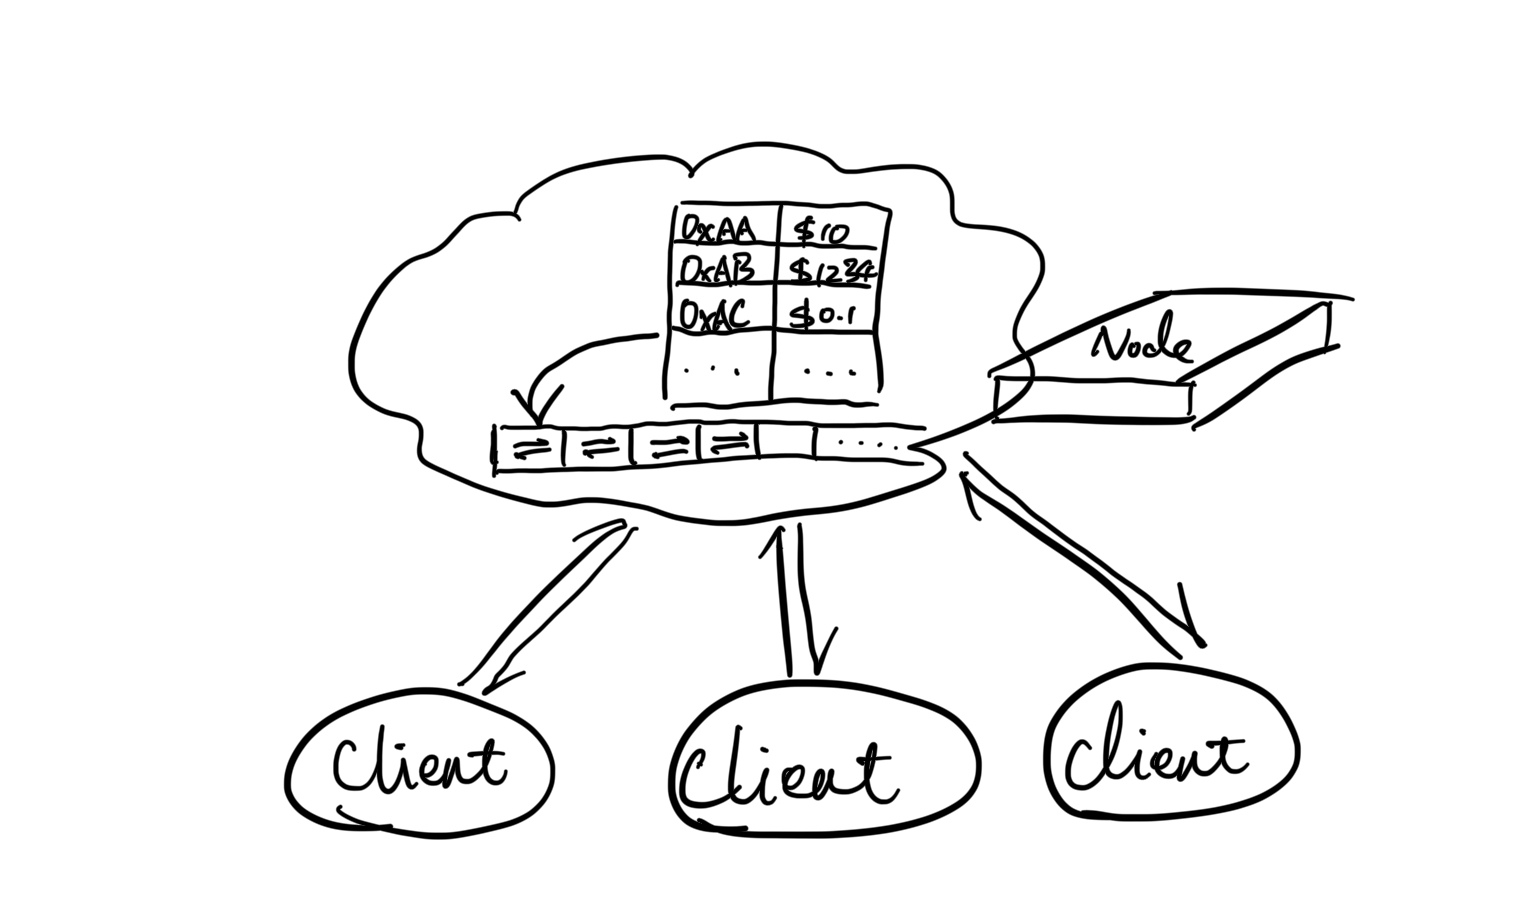
\includegraphics[width=300pt]{graphs/IMG_0050}
    \Description{}
\end{figure}

The upside is the efficiency. Every transition reaches finality in one round trip.
(For bids we consider the finality as the time it is guaranteed to be observable to the other bids.)
Moreover, there's also resource efficiency: the system is running with minimal works being done.
You can literally remove no work but still complete all transactions.
Nothing is wasted.

And the downside has been overly talked.
The centralized operating node can manipulate the market into whatever the node wants it to look like.
Even if directly forging the states can be prohibited (but probably just mitigated) by cryptographic, forging the control path is always doable.
And the most obvious kind of such faults is censorship.

So we move on to the decentralized architecture, prevent single node to have the full control to the ledger.

\begin{figure}[H]
    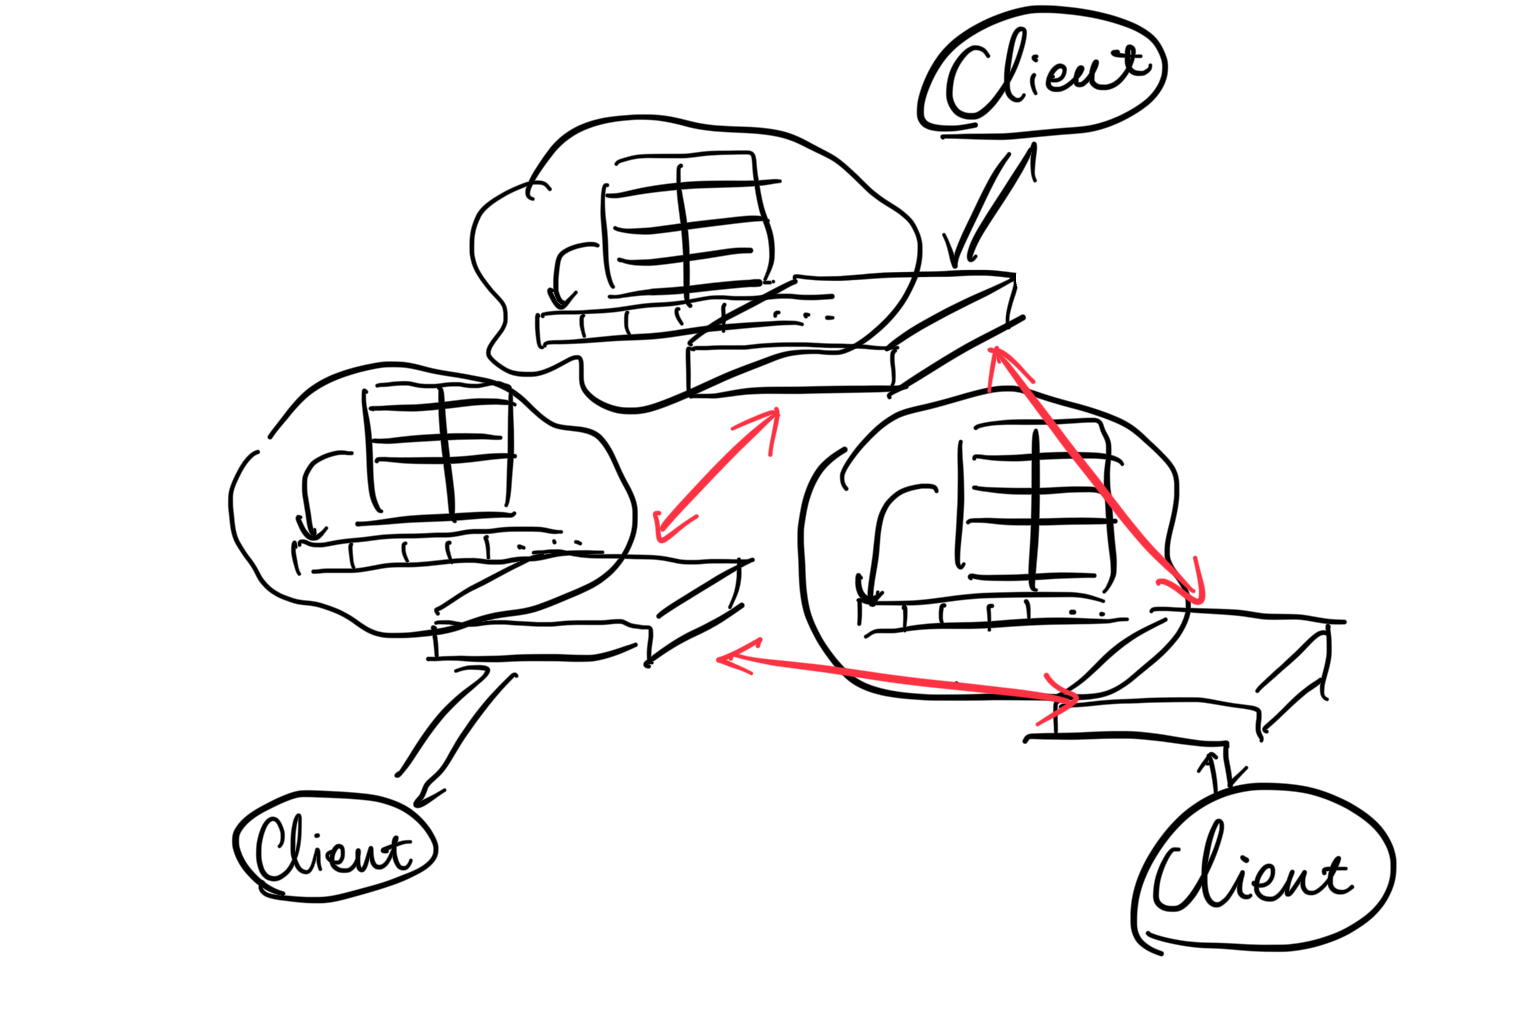
\includegraphics[width=300pt]{graphs/IMG_0051}
    \Description{}
\end{figure}

And we have built a market that cannot be arbitrarily manipulated by (in some definition) minority of the participating powers.

Well, since it's a market it always has some rules.
The rules are usually objective and simple, though you can include a simple ``meta'' rule to allow everyone to add rules so that the running rules may be complicated (but still objective).
The most noticeable property is that all rules \emph{must} be open to everyone.
Only with this property, everyone can \emph{predict} the future ledger states, so they can decide their votes on a candidate running state.

\begin{quote}
    \small
    I don't think zero knowledge is changing this fact.
    While ZKP hides some input to the verifier, the logic skeleton is left in the circuit and must be revealed to the public.
    It is theoretically possible to build circuit acting like an interpreter and put the bytecodes into witness, but then the proof probably loses all the security senses.
\end{quote}

\paragraph{Centralized decentralized market.}
But a market that but be predicted into arbitrary future is uninteresting.
And the unpredictable component has been the \emph{proposers}.
Essentially, it has been the proposers who decide the events to be evaluated according the set of predefined rules, and it has been them to decide the future of the market.
Then how are proposers chosen?
Probabilistically toward the most ``powerful'' ones.
So the future of a decentralized market is eventually based on the subjective opinions of the most powerful participants.
This is the root reason for MEV stuff to be possible: subjective opinions matter in the system.

The ``centralized'' decentralized market did not help us go further enough.
While the decentralization can prevent nodes from manipulating markets in the \emph{absolutely} faulty ways, it cannot rule out all self-beneficial attempts.
The control flows are still with (limited) vulnerability.
And it is unsolvable with the ``define the rules and everyone follows'' approach as long as your rules do not lead to a deterministic future, which is the basic requirement for any useful system (except the ones solving scientific puzzles).

The root cause of such undesirable centralization is the fact that everyone is sharing the same mutable states.

\begin{figure}[H]
    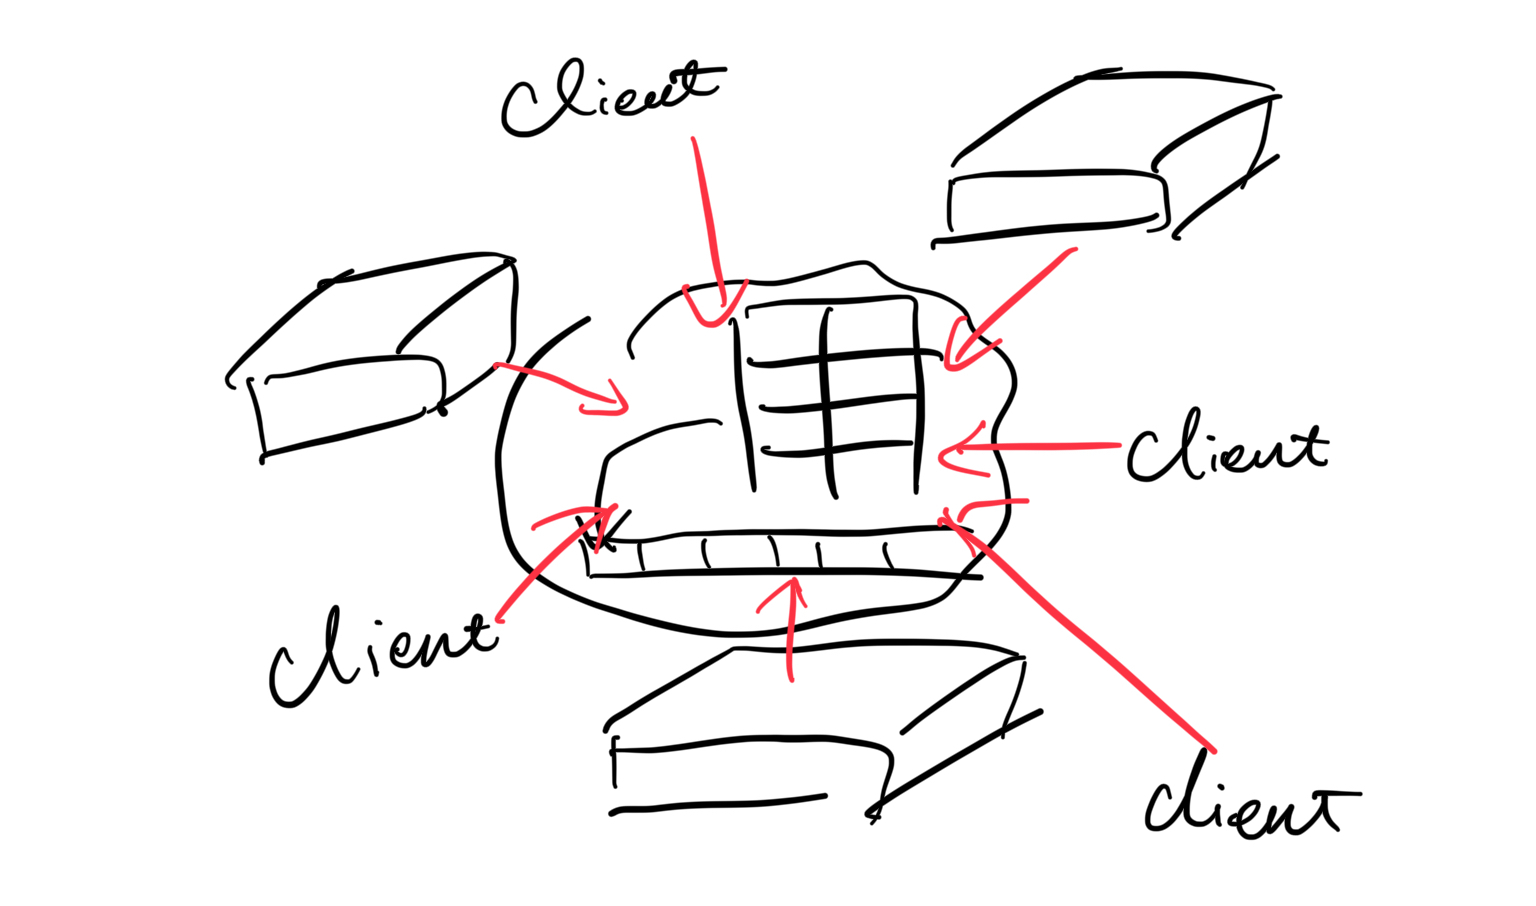
\includegraphics[width=300pt]{graphs/IMG_0061}
    \Description{}
\end{figure}

And every mutation of the states must be initiated by \emph{someone}, instead of objective rules, to enable unpredictable markets.

The current mitigation is to randomize the proposers.
This approach trades security with performance.
The large scope of candidate proposers of a round, the more overhead.
This is a solution that cannot scale.
Moreover, considering we have already traded a lot of performance for just propagating the shared state globally, this approach push us even further from the centralized markets in the sense of performance metrics.
The quantitative differences eventually lead to substantial ones.
There are certain services that widely provided by centralized markets, while impractical/not meaningful as smart contracts because of the poor performance.

Consensus drags.

\section{L1 Sequencer: a Motivated Example of Dedicated Ordering Mechanism}
\sgd{The material here will be a mind experiment.
The details need further polish, and not sure whether it helps in the narrative.
But anyway, it is supposed to be an intermediate step to help understand the ordering/finality separation without involving unfamiliar concepts like partial ordering, brokers, etc.}

\section{Approach}
\label{sec:approach}
\begin{wrapfigure}{R}{0.2\textwidth}
    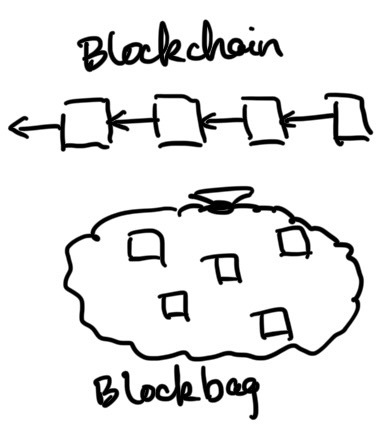
\includegraphics[width=0.2\textwidth]{graphs/IMG_0066}
\end{wrapfigure}

\paragraph{The only-for-finality mechanism.}
The \emph{chain} structure in blockchains corresponds to its inherent ordering functionality.
To clearly draw the difference between them and the finality mechanism in \sys, we explicitly change the representation from ``a chain of blocks'' to ``a (unordered) set of blocks''.
\sgd{Or ``a bag of blocks'' if that is more vivid.}
\sgd{Blockbag? :)}

The \emph{append-only} property of blockchains is expected to be preserved, though.
Anything (or any block) that has been finalized is expected to not get ``de-finalized'' indefinitely.
This property directly enables blockchains to execute the blocks in the finalization order, and \sys also relies on it.
The ``append'' here seems to imply the ordered direction.
Since our finality is unordered, maybe should call it \emph{insert-only}, while the logical clocks are the ones that append-only, to draw a clear distinction.

Since the finality mechanism in \sys requires a subset of blockchains functionalities, blockchains can certainly serve as the finality mechanism.
If necessary we may conduct research on alternative finality mechanisms, but blockchains, especially Ethereum, are probably good enough for now.

\paragraph{What is getting ordered?}
In blockchains it's ``blocks'' that are getting ordered, and inside the blocks it's ``transactions'' that are ordered (subjectively) by the blocks' proposers.
The two-layer design is purely for performance optimization (\ie batching) and has no practical meaning, to we can ignore the outer layer and simply say it's transactions that are getting ordered.

The meaning of \emph{transaction}, though heavily overloaded, probably implies finality.
In \sys what get ordered has no finality (yet).
It is only finalized when it has been submitted to the finality mechanism, not upon ordered.
In another word, they are not transactions ``yet'' upon ordered, and they may or may not ``turn into'' transactions depending on whether they will eventually be finalized.

In the logical clock related introductions we usually put it as it's ``events'' that get ordered.
Since we are describing a financial market solution here I would realize the concept as \emph{quotes}, \emph{preorders} or \emph{letters of intent}, and \emph{intents} to refer them as a whole.
It's probably fine to reuse \emph{transaction} to refer what has been submitted for finality.

\paragraph{The properties of ordering.}
\sgd{If necessary (which probably is), discuss the rationale behind these properties.
What bad things can happen if we don't have them?}
\begin{itemize}
    \item Share-nothing distributed.
    The ordering mechanism itself does not require propagation \ie communication across the whole system.
    In another word, \sys does not forcefully \emph{push} the ordered intents, like how blockchains push the ordered blocks, to the nodes.
    Nodes certainly need to actively \emph{pull} the intents that are involved in the orders they would propose, and that is on demand.
    The system shares nothing more than the minimum.
    \sgd{In previous discussions this has been referred as ``laziness'' or ``lazy consensus''.
    Those words are also not bad in precision, and we can use them if they are better marketing terms.}
    
    \item Optimal parallelization, this is closely related to the previous.
    More than one node can contribute to the ordering concurrently/simultaneously, and if necessary every node can contribute at the same time.
    This is completely on the opposite to the blockchains, where \emph{at most one} node can contribute to the ordering at any time \ie the qualified proposer of the round.

    No matter when, no matter where, no matter whom in the \sys system wants to order no matter what, they can do it \emph{immediately}, without waiting for anything \eg becoming the proposers.
    
    \item Verifiable and append-only.
    These are the revisiting properties of blockchains.
    They are necessary to \emph{preserve} the finality through all ordered intents.
    The following explains this more in action.
\end{itemize}

\begin{wrapfigure}{R}{0.4\textwidth}
    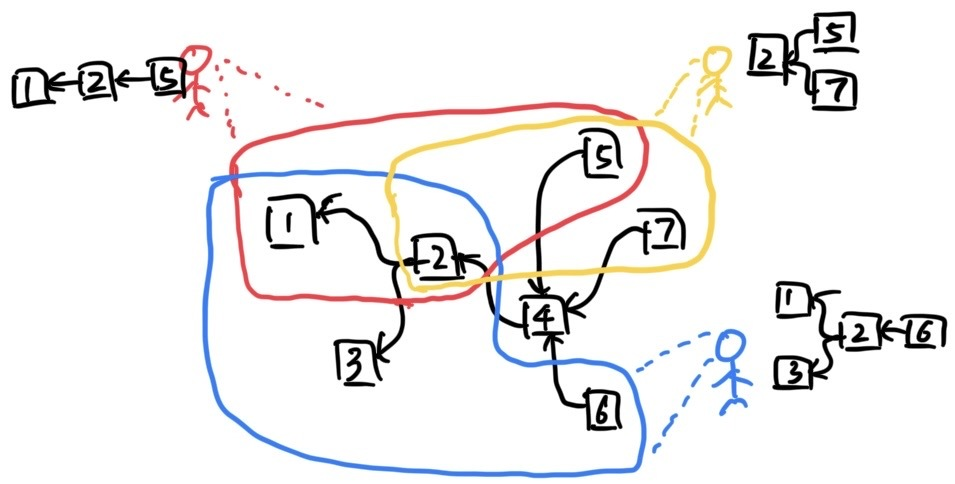
\includegraphics[width=0.4\textwidth]{graphs/IMG_0064}
\end{wrapfigure}

\paragraph{The cooperation.}
The ordering mechanism forms a \emph{partial ordering} among the intents.
Notice that although we represent the partial ordering as a single graph in the illustration, the graph is not shared in reality.
In another word, (probably) no one in \sys actually get to know the whole graph.
Everyone can only learn it partially, according to their point of view.

However, everyone's partial view is guaranteed to be \emph{compatible} to the other's one.
Every partial view is a subgraph of the whole graph.
And if you merge all subgraphs together, you just get the whole graph back, without any risk of confliction.
\sgd{Well, these material may be a bit too technical, try rephrase it more comprehensively.}

\begin{figure}[H]
    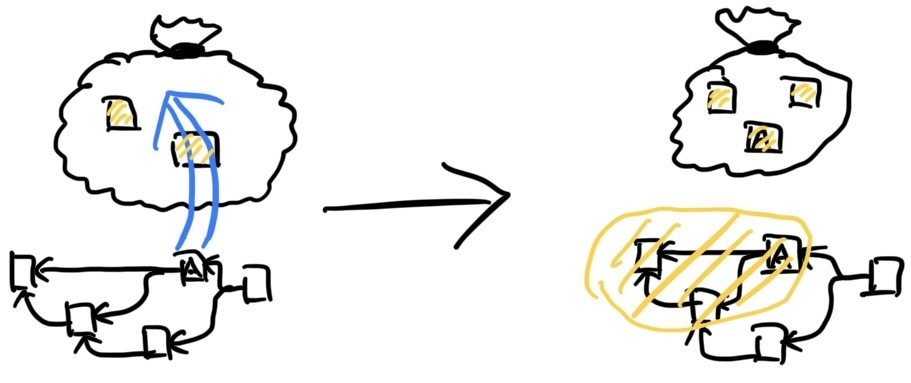
\includegraphics[width=0.5\textwidth]{graphs/IMG_0065}
    \Description{}
\end{figure}

If anyone wants to finalize an intent \ie ``make a deal'' according to it, they submit the intent to finality.
As we stated above, finality mechanism in \sys is an insert-only bag of intents.
Effectively, the finality mechanism \emph{endorses} the intents by inserting them into the consensus bag.
The transitivity of \sys's partial ordering extends the \emph{endorsement} to a larger set of intents.
\sgd{This happens to match the \emph{transitivity closure} concept in mathematic.
(Well, not completely accidentally, I have designed it in this way.)
Make use of this fact if having a proper formalization helps in some way.}

What important is that the extended endorsement is \emph{finalized}.
Although finality mechanism does not explicitly finalize every endorsed intents, it is safe to consider all of them finalized, thanks to the verifiable and append-only properties of the ordering mechanism.
As the result, \sys's ordering mechanism becomes an \emph{amplifier} for finality.
\sys not only enables real time ordering, but also \emph{more} finality.
We believe that nodes can only be incentivized to propose ordered intents that will be finalized (probabilistically), just like they can only be incentivized to propose blocks if the blocks will be chained.
With our ordering mechanism design, the fact that the ordering is not happening inside finality mechanism doesn't change the fact that the ordering still can be finalized, so \sys does not expose challenges in economics.

\sgd{Weird material above, probably fits somewhere else.}

Intents do conflict.
That's why finality does not endorse every submitted intent, but only the \emph{compatible} ones.
What intents are compatible is application specific, which is a topic elaborated in the following section.
In the worst case, intents that do not reside on the same chain all conflict to each other.
Those are the applications that essentially make use of shared mutable states, and they would better directly deploy on blockchains.
We expect our targeted applications to have few contentions on the finality, but every finality involves a lot of collaboration efforts, and the willingness of the collaborations all come with \emph{preconditions}, or assumptions.
This sounds a lot abstract, but as shown below, finance can be one such case.

\sgd{Personally I'm already satisfied by describing ``what we are good for'' in one sentence, regardless of the abstractness.}

\section{Case Study: Decentralized Finance}
\label{sec:finance}
\paragraph{System overview.}
The imagined financial market is a lot like what crypto exchanges can do today.
Users mostly trade tokens and their derivatives in the market.
Trading offchain merchandises are possible, and the security mechanism is nothing particular to today's offchain solutions \eg producers submit a proof of finished the work to the chain and get rewarded from smart contracts, or challengers submit a proof of producers not finishing the work to the chain to get slashing rewards from smart contracts.

The users are categorized into \emph{dealers} and \emph{customers}, based on whether they are providing offers or accepting ones.
Dealers may not be (long) sellers; they can on short position and provide offers to buy merchandises from the others.
We will use the standard terms of \sys in the following discussion.
The dealers are further categorized as \emph{producers} who produce the (chains of) quotes (either for sale or purchase), and \emph{broker} who produce derivatives.
The customers are called consumers.

For simplicity, we only discuss trading onchain merchandises here, and we only consider deploying to Ethereum, so the tokens would be ERC-20s and NFTs.
Those are directly transact-able on Ethereum through interacting with smart contracts, and the advantages of \sys mirrors the ones stated in our vision:
\begin{itemize}
    \item Real time. 
    It's not as simple as ``the transaction can be made faster''.
    Because the transaction eventually still happen on the chain, and we are not doing things like preconfirmation to assure anything.
    The ``real time'' here means real time reaction.
    \sys allows user to action much more frequently than the finality frequency, and those are additive actions that eventually contribute to the \emph{same} finality.
    More details later.
    \item Heterogeneous.
    In plain Ethereum system brokers are homogeneous \ie they are just smart contracts.
    In \sys how brokers work is completely unspecified.
    It's all hidden to the blockchain.
    \item Intersubjective.
    \sgd{This one I haven't got it clear. Skip for now.}
\end{itemize}

\paragraph{Advantage over current L1 exchanges.}
They are centralized.

\paragraph{Design overview.}
Most of the communication/``brokerage''/potential negotiation happens offchain.
The intermediate ``intents'' are accumulated with logical clocks.
As soon as the intents are turning into a ``deal'', the payers submit the final logical clocks and their payments to the smart contract for finality.
After the finality, the payee(s) also consult the smart contract with their logical clocks as proof to receive their rewards.
These consultations can be made asynchronously and periodically batched, to reduce the overhead of interacting with the chain.

\paragraph{Example: a deal.}
The producer sells an NFT A for 1ETH.
It (offchain) publishes a quote intent (A = 1ETH).
The consumer buys the NFT, by submitting to \sys smart contract with the (logical clock of) quote intent and 1ETH.
The producer later submits to \sys smart contract with the same logical clock (and the smart contract is able to verify that the producer is the owner of the clock) and receive 1ETH from the contract.
The contract also transfer the ownership of NFT A to the consumer.

In this minimal case there's no benefit of making use of \sys.
A simple smart contract that transfers both NFT and ETH will conclude the interaction in single transaction.

\paragraph{Example: a match.}
Producer 1 sells 1ETH for 3500USDT.
\sgd{Current market price from Google.}
Producer 2 buys 1ETH with 3501USDT.
The consumer generates a match intent with a logical clock merging both quotes, and sends it to producer 2.
Producer 2 submits to \sys smart contract with 3501USDT payment.
Later producer 1 and consumer individually consult the contract and get 1USDT and 3500USDT respectively.
Consumer also transfers 1ETH to producer 1 during the consultation.

\sgd{Why producer 2 should submit the transaction, not producer 1 or consumer?}
\sgd{Why pays 3501USDT not 1ETH?}
\sgd{Is this a consumer or broker? Are these producers or consumers?}
\sgd{I'm not good at designing a market...}

In comparison, with plain Ethereum the matching engine will be a smart contract \eg uniswap.
The matching logic is public and (what's worse) it must be expressible with smart contract.
You cannot perform a subjective matching, not even an intersubjective one.
And further, producer 1 and producer 2 need to both interact with the matching contract.
That probably cannot take place in the same block (without any speculation).
However in \sys they may have adjusted their quotes for arbitrary many times before the matching is accomplished, and all those communications can happen right within 12 seconds.

\paragraph{Example: a derivative.}
\sgd{Work in progress.
Not sure whether it's necessary to have one more example.
A single-layer derivative should be much similar to the match, and a more deeply nested one would be too complicated to illustrate.}

\paragraph{What is ordered? (again)}
There are different concepts of \emph{ordering} in a financial system.
Although we can generalize all of them into ``A only if B'' form, but it's worth to perform a case study.

The first kind is temporal ordering.
Consider the price of certain merchandise.
It changes, and the current price is certainly \emph{after} its price from previous timestamp.
In \sys we represent the quote intents as ``conditional quotes with expiration''.
The interpretation is ``the price of the merchandise is \$X, and the price is only valid 1. before the current block (hashed Y) reaches depth Z in the chain and 2. all previous quotes of the merchandise were not finalized''.
Finality mechanism checks for the requirements before endorsement, to prevent a merchandise to be sold more than once.
The producers may repeatedly propose quotes for their merchandises until they are sold.

The second kind is derivative ordering.
An index intent can be ``the price of the index is \$X, and the price is only valid while all indexed quotes are valid''.
\sgd{Intents for options can be a bit more tricky, since it involves quote intents that will be proposed in the future.
We can design for them later.}
Notice that all of these are not actually transactions, but instead somehow ``I would like to transact with X if Y would like to transact with me''.
The ``letters of intent'' in this form are perfectly composable and can be arbitrary nested.
When a highly-nested intent is finalized, a lot of intermediate transactions are finalized at once.
In a blockchain system all these intermediate steps have to happen on chain, incurring high latency and lots of gas overhead.
While in \sys, only one intent is submitted for finality regardless of the number of intermediate steps.
This means perfect scalability.

The last kind is transaction ordering.
This is the ordering of mutating states.
If two consumers buy the same merchandise, the transaction ordered first will success and the other one must be aborted.
In the baby step described in this working document, the market states are remained on chain (though a lot of intermediate states are skipped), so such ordering corresponds to the ordering of finalization.
\sys is not responsible for it and simply leaves it on the chain.

There will be parallelization opportunities to explore in the transaction ordering.
As a patch we may design certain derivative to ad-hoc bundle transactions into ``mega-transactions'', which make profit by reducing gas fee during finality.
Don't know for sure whether that works.

\paragraph{Current limitations.}
There's no offchain computation in current design.
Actually, all offchain states are intermediate, ephemeral and fine to be unreliable.
\sgd{probably}
Since financial is neither computational heavy (in the sense of \emph{processing transactions themselves}, not \emph{making decisions of transacting or not}) nor data heavy (ideally just one balance number per account), going offchain may not benefit much.

However, not persisting states outside the chain also means we will not have our own economics.
The settlements will be in ERC-20 and there's no necessity to roll out our own token.
I think we probably still can make money in some way without our own token, but others (probably) may not.

And after all, this is contrary to the vision states previously \ie blockchains as unordered finality, nothing more.
It's more like an incremental contribution to current blockchain systems \ie yet another offloading/rollup solution (while substantially differs from current rollups).
This is good for bootstrapping, but we probably should move on later.

\paragraph{Sketch of smart contract design.}
The contract's main task is to verify logical clocks.
The verification results come with the determined ordering, and specific verification semantics should be integrated case by case.
Finally, the contract is the temporal token holder for outstanding transactions, to enable asynchronous interaction with the chain.
\sgd{Also enable us to make money from the system.}

Take calls for an example.
The consumer interacts with blockchain first, submits an intent of either a quote or a derivative of some intents, indicating that the consumer is willing to call with certain amount of tokens.
The contract performs several checks, including whether the intent is equipped with a valid logical clock, whether the call conflicts with previous calls, and the other ordinary checks \eg whether consumer account has sufficient balance.
If all checks pass, the contract transfer the tokens from consumer account to the contract account, and finalize the intent.

% \paragraph{Check for confliction.}
% The smart contract maintains a logical clock in the chain state.
% Upon endorsing an intent, the contract merges it into its onchain clock.
% At the result, if a submitted transaction conflicts with previously finalized ones, its clock will 

\sgd{Work in progress.}

\section{Case Study: Collaborative AI}
\label{sec:ai}
\paragraph{Motivation and system overview.}
The end users of AI market consumes AI services/products \eg conversation sessions, content generation, etc.
Currently, the services are \emph{scheduled} / \emph{orchestrated} / \emph{assembled} mostly by single party.
\sgd{Having difficulty choose the best word...}
In another word, there's a centralized participant that contacts all the other participants in the systems, namely GPU owners, model creators, and end users.
This one-stop architecture does not enable the full competition market and the optimal configuration of resources.

The root cause of today's centralized architectures is the difficulties of efficiently collaborate in real time.
Suppose A users own GPUs and B users owns models.
Without further assistance, it is hard for the individuals of either A users or B users to \emph{ad hoc} find each other in real time that \emph{matches} \ie the GPUs must be capable to inference the models.
Both of them cannot fulfill user demands alone.
As the result, the cooperation must be negotiated ahead of time and be longstanding, which in turn requires heavier trust mechanism \eg staking.

In \sys none of the participants need to take care of the whole workflow.
The consumers, brokers and producers concept from \autoref{sec:finance} are also applied in this case.
The producers provide GPUs and other AI hardware.
The consumers purchase AI services by contacting one of the brokers who announce to provide the services.
Those brokers, however, provide end user services based on the model inference services provided by other brokers.
And those brokers that support inference rent the hardware from producers.
The logical clocks, which order the intents all over, enable such collaboration despite every participant only works locally.

\paragraph{Example: oneshot query.}
Producer A announces intent of 10s GPU time for 1USDT.
Broker B announces a conditional intent of ``as long as A fulfills its intent to me, I provide a llama model inference of any input for 1.01USDT''.
Broker C announces a conditional intent of ``as long as B fulfills its intent to me, I can answer a professional question for 1.02USDT''.
(C achieves this by sending special prompts to the model during inference.)
Consumer D thinks ``ok I have a computer science professional question to ask and I'm willing to pay 1.02USDT''.
Then D submit the intent announced by C and 1.02USDT to the \sys smart contract on the chain.

After C's intent has reached finality on the chain, C takes D's question, combined with its special prompts that can make llama model act as a computer science professor, together send to B.
B then perform inference with its llama model on A's GPU.
After the task is done and the proof of work is generated (or after a while no one challenges that the work is not done correctly), A, B and C interact with \sys contract on the chain with their original intent logical clocks.
The contract verifies their logical clocks are based by the one submitted by D (or is the same one, for C's case).
And transfer corresponded tokens according to the intents.
Thus, A, B and C receives 1USDT, 0.01USDT and 0.01USDT each.

\paragraph{What are the clocks used for?}
Logical clocks are crucial in the workflow above for multiple purposes.
\begin{itemize}
    \item B, C and D verifies the \emph{single} logical clock from its immediate predecessors, and conclude that \emph{all} previous intents are verified.
    \item Smart contract verifies A, B and C's clocks, and the relation between their clocks and the D's one, conclude that they should be paid.
    \item A, B and C can interact with the smart contract in arbitrary order, arbitrarily after the transaction was finalized (\ie D submitted).
    \sys removes the necessities of \emph{synchronously} interact with the chain for all the intermediate steps.
\end{itemize}

Other than constructing conditional intents, the clocks can also be used for local ordering.
For example, A may announce intents of every 10s of its GPU times, and each intent is ordered after the previous one.
So that if another broker E has its intent based on a latter intent of A (based on A's ordering), then E can only utilize A's GPU after B is done.

\paragraph{Discussions.}
There's no security model here.
In reality we need to specify one, even if it's ``yes we don't have security'' that still need to be decided.

The division of GPU providers and model providers are impractical.
If models must be sent to GPUs owners in clear text, models will not be confidential, and that's a lot of network overhead.

\bibliography{paper}
\end{document}
